
\chapter{The Lifshitz model: general presentation.}

\section{The Lifshitz model and its main features}

\subsection{The Lifshitz model}

\subsubsection{The modulated phase and the Lifshitz phase diagram.}


In the modulated phase (fig. \eqref{fig:evol_strip}) typical the Lifshitz model, the order parameter is spatially periodic in one or several directions of space. We will label with a $\sslash$ sign quantities living in these directions, and $\perp$ the quantities living in the orthogonal subspace.

\begin{figure}[htp]
\centering
\begin{subfigure}{.33\textwidth}
	\centering
	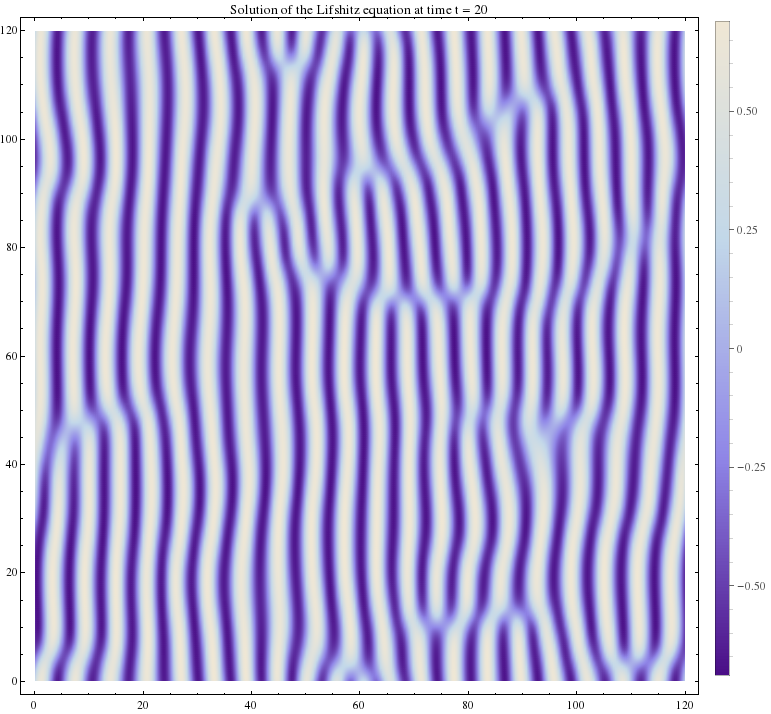
\includegraphics[width=.9\linewidth]{img/chap1/sol_Lif_t20.png}
	\caption{}
	\label{lif_t20}
	\end{subfigure}%
\begin{subfigure}{.33\textwidth}
	\centering
	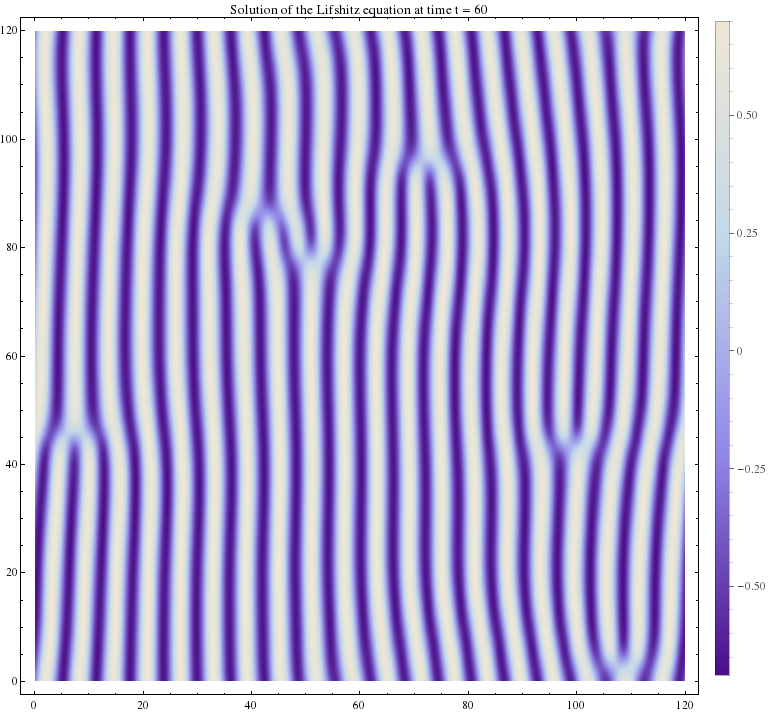
\includegraphics[width=.9\linewidth]{img/chap1/sol_Lif_t60.png}
	\caption{}
	\label{lif_t60}
\end{subfigure}%
\begin{subfigure}{.33\textwidth}
	\centering
	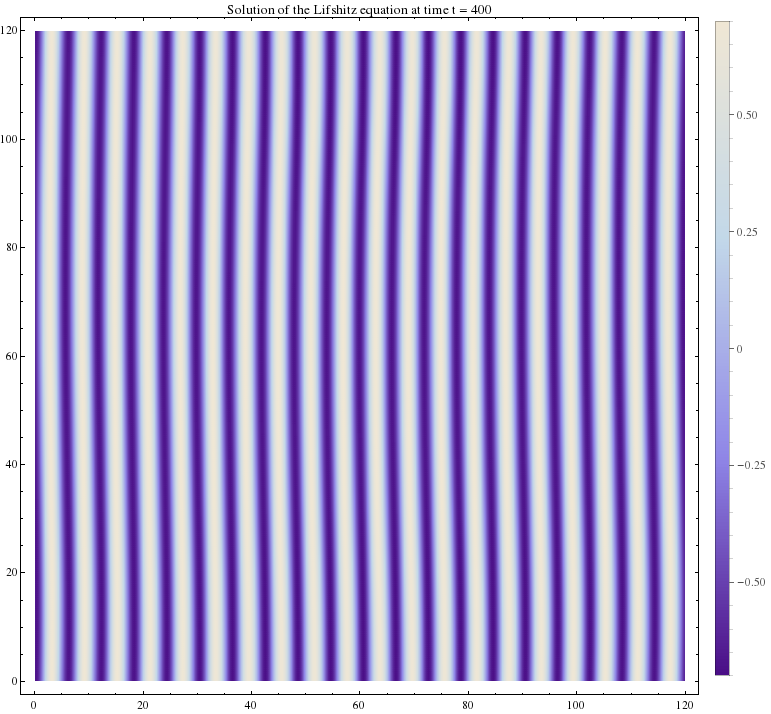
\includegraphics[width=.9\linewidth]{img/chap1/sol_Lif_t400.png}
	\caption{}
	\label{lif_t400}
\end{subfigure}
\caption{Time evolution of a field obeying the equation of movement derived from the (time dependent) Lifshitz action. We see that the structure evolves toward a modulated steady state.}
\label{fig:evol_strip}
\end{figure}


Typically, the phase diagram of such a physical system will resemble the one presented in fig. \eqref{fig:phase_diagram}.
\begin{figure}[htp]
\begin{center}
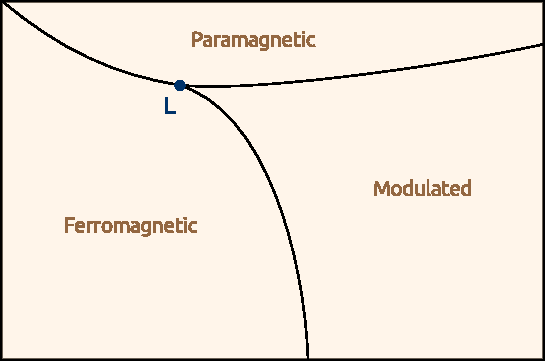
\includegraphics[scale=1]{img/chap1/phase_diagram_2.pdf}
\caption{Typical phase diagram of a system described by the Lifshitz model. The Lifshitz point is labelled $L$. Temperature varies along the vertical axis while the horizontal axis accounts for the variation of an extra parameter $\rho_0$.}
\label{fig:phase_diagram}
\end{center}
\end{figure}

A crucial feature of this phase diagram is the intersection point of the modulated, ferromagnetic and antiferromagnetic phases, called the Lifshitz point ($L$ in fig. \eqref{fig:phase_diagram}). 
Historically, the manganese phosphite (MnP) magnetic crystal was one of the first systems in which a Lifshitz point could be detected. Moreover, the entire phase diagram around the Lifshitz point of the MnP crystal could be inferred with high precision from experimental measurements \cite{MnP}.
The phase diagram of a Lifshitz system is bidimensional: one axis being the temperature, and the other and extra parameter -- called $\rho_0$ from now on, whose precise meaning depends on the physical nature of the studied system.
In the case of the MnP magnetic crystal, the tunable $\rho_0$ parameter is an external magnetic field applied to the crystal, while the order parameter  is the magnetic moment of the atoms. In the modulated phase, it is the angle between the direction of the magnetic moment and a direction of reference that is spatially modulated.

Experiments also provide evidence of Lifshitz point existence in ferroelectrics and liquid crystals.

\subsubsection{The Lifshitz model}

The Lifshitz model is a field theory, describing a vector field $\boldsymbol{\phi}$ whose components will be denoted $\phi_i$.
If we like to think in terms of magnetic systems, like the MnP cristal, we can say that $\boldsymbol{\phi}(x)$ is the coarse-grained magnetization at position $x$.
 To write the action for the Lifshitz model, we choose a basis $(\mathbf{e}_n)_{1 \leq n \leq d}$. We decide that this basis is such that its first $m$ vectors span the $m$ dimensional $\sslash$ subspace, while of course the remaining $d-m$ base vector span the $\perp$ subspace. In this basis, the Lifshitz action is
\begin{equation}
S = \int_x \sum_{i=1}^N \left( \frac{1}{2} \left(\sum_{n_\perp=m+1}^{d}\frac{\partial \phi_i}{\partial x_{n_\perp}} \mathbf{e}_{n_\perp}\right)^2 + \frac{\rho_0}{2} \left(\sum_{n_\sslash=1}^{m}\frac{\partial \phi_i}{\partial x_{n_\sslash}} \mathbf{e}_{n_\sslash}\right)^2 + \frac{\sigma_0}{2} \left(\sum_{n_\sslash=1}^{m} \frac{\partial^2 \phi_i}{\partial x_{n_\sslash}^2} \mathbf{e}_{n_\sslash}\right)^2 \right) + U(\phi)
\end{equation}
As we want to model the broadest possible class of physical systems, we will say that $U$ is an almost completely arbitrary potential. We only ask for it to have the $O(n)$ symmetry, \textit{i.e.} to be a function of $\rho \define \phi_i \phi_i/2$.

From now on we will use the self-explanatory shorthand notation
\begin{equation}
H[\phi] = \int_x \left( \frac{1}{2}(\p{\perp} \phi)^2 + \frac{\rho_0}{2}(\p{\sslash} \phi)^2 + \frac{\sigma_0}{2} (\p{\sslash}^2 \phi)^2 + U(\rho) \right)
\end{equation}

We see that this action closely resemble the well known action of the $O(n)$ model
\begin{equation}
S_{O(N)} = \int_x \left( \frac{1}{2}(\partial \phi)^2 + U(\rho) \right)
\end{equation}
Namely, we recover it if we set $\rho_0 = 1$ and $\sigma_0 = 0$. We see that what differentiates the Lifshitz and $O(n)$ action is on one hand the presence a non trivial (\textit{i.e.} different from 1) $\rho_0$, breaking the $O(d)$ invariance, and on the other hand the presence of an extra term involving a Laplacian squared. Clearly, these two modifications must be responsible for the appearance of spatially modulated structures, but why exactly? 
We can gain a useful intuition of why a spatially modulated structure is closely linked to the existence of a Laplacian squared term in the action by looking at a microscopic version of our model. 

\subsection{A discrete counterpart: the anisotropic Ising model}

Stricto sensu the discrete counterpart of the Lifshitz model would be an anisotropic Heisenberg model, but to simplify things -- without changing the essence of the argumentation -- we consider an anisotropic Ising model instead.

First, let us consider a chain of Ising spins with the Hamiltonian
\begin{equation}
H_{\text{chain}} \define - J \sum_i S_i S_{i+1}
\end{equation}
We know that if $J$ is positive, the interaction is ferromagnetic, whereas is $J$ is negative, the interaction is antiferromagnetic. 
The antiferromagnetic order already shows some kind of spatial modulation, but it only exists at zero temperature! 
The idea to make a spatially modulated order survive at non zero temperatures is to consider a second neighbors \textit{antiferromagnetic} interaction, together with a first neighbors \textit{ferromagnetic} interaction:
\begin{equation}
H_{\text{chain}} = - J_1 \sum_i S_i S_{i+1} - J_2 \sum_i S_i S_{i+2}
\end{equation}
However, for a long range order to exist at finite temperature, we need to work in two dimensions or more, \textit{i.e.} to trade our spin chain for a spin lattice:
 \begin{equation}
 H_{\text{lattice}} \define - \sum_i \left( J_0 \sum_{\delta_\perp} S_i S_{i+\delta_\perp} + J_1 \sum_{\delta_\sslash} S_i S_{i+\delta_\sslash} + J_2 \sum_{\delta_\sslash} S_i S_{i+2 \delta_\sslash} \right)
 \end{equation}
 Qualitatively, the competition between ferromagnetic and antiferromagnetic interactions will produce a spatial modulation of the spins at non zero temperature, at least for some values of the interaction strengths ratio $J_2/J_1$. 
 The existence of a stripped phase indeed is a well known feature of this model \cite{ANNNI}, called the ANNNI (axial next-nearest neighbour Ising) model.
 
 Now, what is the link between this discrete spin lattice Hamiltonian, and our continuous action?
Note that a sum on nearest neighbors can be rewriten in terms of a discrete Laplacian on the lattice, while a sum on next-nearest neighbors involves a discrete Laplacian squared:
\begin{equation}
H_{\text{lattice}} = -\sum_i \left( \kappa S_i^2 + J_0 S_i \Delta_\perp S_i + (J_1 + 4 J_2) S_i \Delta_\sslash S_i - J_2 S_i \Delta_\sslash^2 S_i \right)
\end{equation}
where we introduced the differential operators on the lattice:
\begin{align}
\Delta_\sslash S_i = \sum_{\delta_\sslash} S_{i-\delta_\sslash} - 2 S_i + S_{i+\delta_\sslash} \\
\Delta_\perp S_i = \sum_{\delta_\perp} S_{i-\delta_\perp} - 2 S_i + S_{i+\delta_\perp} \\
\Delta_\sslash^2 S_i = \sum_{\delta_\sslash} -S_{i-2\delta_\sslash} +  4 S_{i-\delta_\sslash} - 4 S_i + 4S_{i+\delta_\sslash} - S_{i+2\delta_\sslash}
\end{align}
This rewriting in terms of discrete differential operators makes it clear that this Hamiltonian is the discrete -- microscopic -- counterpart of the Lifshitz action. We now understand -- at least intuitively -- the origin of the spatially periodic structures (shown in fig. \eqref{fig:evol_strip}) the field of the Lifshitz model exhibits. They exist because of the competition between \textit{nearest neighbors ferromagnetic interactions} (giving rise to the $\Delta_\sslash$ term in the Lifshitz action), and \textit{next-nearest neighbors antiferromagnetic interactions} (giving rise to the $\Delta_\sslash^2$ term in the Lifshitz action).

At this point a question arises: why work with a Lifshitz coarse-grained field theory, since we have a better physical understanding of an underlying microscopic model? What is more, in passing to a continuous theory, we lose information about the microscopic underlying lattice. 
This is actually not a problem since the statistical quantities we are interested in computing -- namely the critical exponents of the phase transition -- are universal; they do not depend on the specific microscopic model, if the symmetries of this model were carefully implemented in the continuum limit. Actually, passing to a field theory is even advantageous as it frees us of the irrelevant microscopic details. 
Even more crucial is the fact that field theories are the objects of choice for application of the powerful methods of the renormalization group, which we will now describe.